\documentclass{article}

% if you need to pass options to natbib, use, e.g.:
%     \PassOptionsToPackage{numbers, compress}{natbib}
% before loading neurips_2021

% ready for submission
\usepackage[preprint]{neurips_2021}

% to compile a preprint version, e.g., for submission to arXiv, add add the
% [preprint] option:
%     \usepackage[preprint]{neurips_2021}

% to compile a camera-ready version, add the [final] option, e.g.:
%     \usepackage[final]{neurips_2021}

% to avoid loading the natbib package, add option nonatbib:
%    \usepackage[nonatbib]{neurips_2021}

\usepackage[utf8]{inputenc} % allow utf-8 input
\usepackage[T1]{fontenc}    % use 8-bit T1 fonts
\usepackage[colorlinks=true]{hyperref}       % hyperlinks
\usepackage{url}            % simple URL typesetting
\usepackage{booktabs}       % professional-quality tables
\usepackage{amsfonts}       % blackboard math symbols
\usepackage{nicefrac}       % compact symbols for 1/2, etc.
\usepackage{microtype}      % microtypography
\usepackage{xcolor}         % colors
\usepackage{siunitx}
\usepackage{graphicx}

\newcommand{\todo}[1]{{\color{red} #1}}

\title{Spotify feat. Logistic Regression - \\ Popularity, Nothing Else Matters}

% The \author macro works with any number of authors. There are two commands
% used to separate the names and addresses of multiple authors: \And and \AND.
%
% Using \And between authors leaves it to LaTeX to determine where to break the
% lines. Using \AND forces a line break at that point. So, if LaTeX puts 3 of 4
% authors names on the first line, and the last on the second line, try using
% \AND instead of \And before the third author name.

\author{%
  Sebastian Hoffmann\\
  Matrikelnummer 5954377\\
  \texttt{sebastian.hoffmann@student.uni-tuebingen.de} \\
  \And
  Yannick Streicher\\
  Matrikelnummer 5331817\\
  \texttt{yannick.streicher@student.uni-tuebingen.de} \\
}

\begin{document}

\maketitle

\begin{abstract}
  What is the musical taste of the world? With the recent rise and global pervasiveness of music streaming services, such as Spotify, Deezer, or Apple Music, answering this question has become tractable. For this, we plan to analyze a \href{https://www.kaggle.com/rodolfofigueroa/spotify-12m-songs}{subset of 1.2 million songs} scraped from Spotify. However, this dataset lacks crucial information about popularity. Thus, an important step of our work is to augment the dataset further by querying the official Spotify REST API for a randomly sampled subset of the data. Besides a birds-eye overview of the musical landscape, e.g. distribution of genres, we want to identify common musical properties shared by popular songs, and likewise, very unpopular songs, using logistic regression. Such properties can be, for instance, tempo, mode, or key.
\end{abstract}

\section{Introduction}
The questions we want to answer during our project are: ""

\section{Methods and Data Collection}
To pursue our overall goal of predicting the popularity of a song given its Spotify features, we have to find good labels that discriminate popular and unpopular songs. However, the Kaggle dataset\footnote{include link} only contains musical song features. Spotify\footnote{link company} includes some metrics that summarize a measure of popularity, derived by preferences of Spotify's users. In the end, two metrics are important for our project, \textit{(i): Popularity:} An integer between 0 and 100 describing how popular a track is. According to Spotify's API description, this metric is determined algorithmically based on the total number of plays a track has, as well as, how recent those plays are. Artist popularity is derived from the popularity of its individual tracks. The second feature is \textit{(ii): Followers} which is the number of accounts that subscribed to this artists Spotify feed. The number can be interpreted as peoples interest in following the new releases of a particular artist.

The starting point for the project was the 1.2m song dataset on Kaggle. For all of those songs, we queried the Spotify API for additional artist information. In total, we queried around \num[]{85 000} artists, each having a popularity score and a number of followers. Additionally, each artist is described by a set of genres.

\paragraph{Filtering and Preprocessing}
With the advent of online self-publishing, it has became very easy and accessable to distribute home-produced music to a worldwide audience. In fact, there exist specialized companies, such as TuneCore or DistroKid for instance, that automatically distribute submitted songs to multiple platforms at the same time, including Spotify and Apple Music. Indeed we find that a quarter of artists on Spotify have less than $45$ followers and half of all artist have less than $393$. For comparison, \emph{Merikan}, a relatively unknown \emph{Drum and Bass} producer, which is not a major genre, has $4581$ follower at the time of writing. Given that self-published songs do not undergo the feedback and quality control process a regular music label would provide to an artist, we are worried that these tracks can potentially introduce a lot of noise to our data. Consequently, we filter our dataset to only include songs of artists that are to some extent known and established and can be considered professional or semi-professional musicians.

There are two metrics that could potentially be considered as a filter criterion: The popularity of an artists and the number of followers. We find that the number of followers is roughly exponentially distributed. After transforming it logarithmically, there is a clear linear relationship between the number of (log) followers and popularity visible (Pearson correlation coefficient: $0.88$, see Figure~\ref{fig:filtering}~left). This indicates that a more robust measure can be derived by combining both metrics into one.

To this end, we transform both followers and popularity using PCA. The first principal component can be seen as a robust measure of artist popularity, whereas the second component indicates the deviation from the linear relationship. Upon further inspection, we find artists such as \emph{\todo{find the minecraft guy}} that while having a significant amount of followers, do not have any successful songs. To further reduce noise, we filter these outliers as well by thresholding the second principal component. This affects $1366$ artists ($1.6\%$). We then threshold the first component to filter $50\%$ of all artists. Finally, we filter all are artists that do not have a genre associated with them (affects $52.26\%$\footnote{Notice that there is a big overlap with unknown artists, presumably since scarce data makes it difficult for Spotify to establish a genre.}).

In total, if all three steps are applied, $62.8\%$ of all artists are removed from the dataset and $31694$ artists in total are retained. This reduces the number of songs left in the dataset to $755472$, or $62.75\%$ of the original size.

\begin{figure}
  \centering
  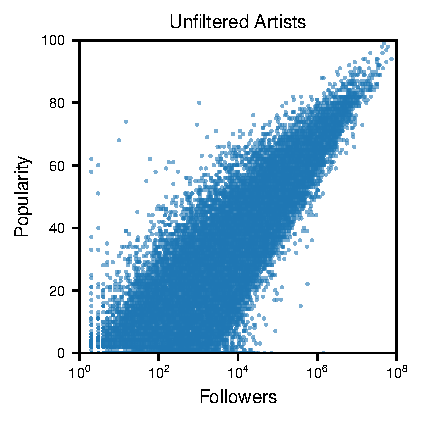
\includegraphics[width=0.42\textwidth]{../figures/artists_unfiltered.pdf}
  \qquad
  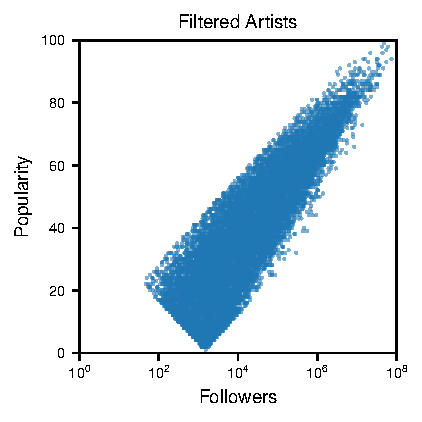
\includegraphics[width=0.42\textwidth]{../figures/artists_filtered.pdf}
  \caption{artists}
  \label{fig:filtering}
\end{figure}

\begin{figure}
  \centering
  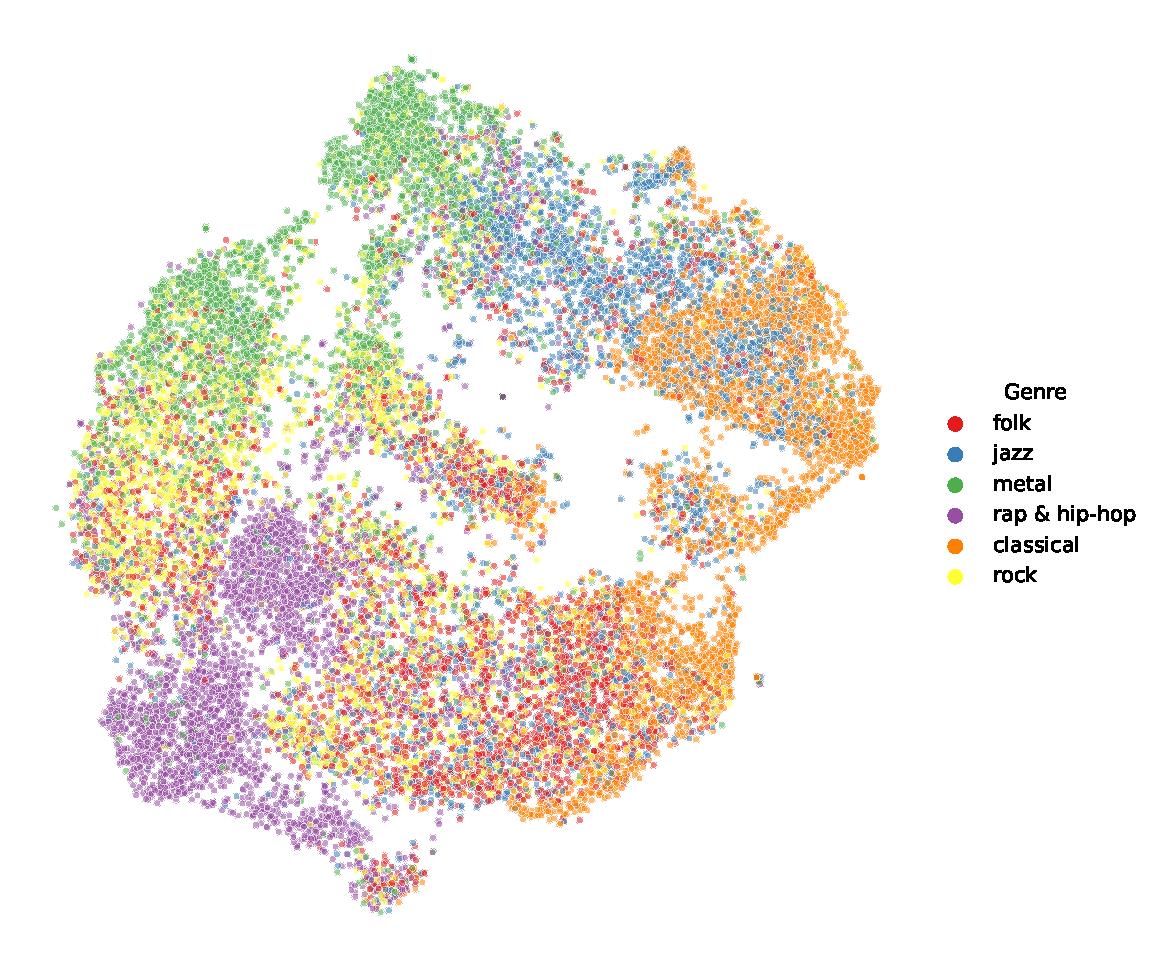
\includegraphics[width=\textwidth]{../figures/tsne_genres.pdf}
  \caption{tsne}
  \label{fig:tsne_genres}
\end{figure}

\begin{itemize}
  \item Starting point: the 12m songs dataset
  \item Query the rest Api for each song to obtain its popularity metrics
  \item Query the rest API for each artist of those songs to obtain Artists followers and popularity scores. Note: this is much less than the songs -> easier first overview
  \item 
  \item Popularity is equally skewed.
  \item Popularity and followers are highly correlated! Maybe consider doing a PCA-like transformation to get a singular and corrected value. Notice as well, that there are some artist that are highly unpopular while still having a significant amount of followers. Are these dead people? Lets find out :)
  \item Include probably famous people from platform like youtube or insta, but who are shitty musicians. For instance, minecraft troll song (Lachlan - Mobs cant handle me).
  To filter these "indie artists", simply thresholding 'followers' or 'popularity' is not sufficient. Instead we need a PCA to remove the outsider of the distribution.
\end{itemize}

\section{Data Analysis}

\subsection{Explorative Data Analysis}

\subsection{Dimensionality Reduction}

\subsection{Statistical Analysis}
For doing ... we applied logistic regression

\section{Discussion}
Our work is limited because\dots
In regards to ... we cannot estimate confidence because ...

\end{document}
